%
% File emnlp2016.tex
%

\documentclass[11pt,letterpaper]{article}
\usepackage{emnlp2016}
\usepackage{times}
\usepackage{url}
\usepackage{amsmath}
\usepackage{breqn}
\usepackage{latexsym}
\usepackage{pgfplotstable}
\usepackage{algorithm2e}
\usepackage{hhline}
\usepackage{multirow}
\usepackage[font=small]{caption}
\usepackage{subcaption}
%\usepackage{hyperref}
\usepackage{color}
\usepackage{lipsum,adjustbox}
\usepackage{tikz}
\usepackage{tikz-dependency}
\usetikzlibrary{shapes,fit,calc,er,positioning,intersections,decorations.shapes,mindmap,trees}
\tikzset{decorate sep/.style 2 args={decorate,decoration={shape backgrounds,shape=circle,
      shape size=#1,shape sep=#2}}}

\setlength{\belowcaptionskip}{-10pt}
\newcommand{\oa}[1]{\footnote{\color{red} #1}}
\newcommand{\daniel}[1]{\footnote{\color{blue} #1}}
\newcommand{\com}[1]{}
\newcommand{\secref}[1]{Section~\ref{#1}}
\newcommand{\figref}[1]{Figure~\ref{#1}}
\newcommand{\tabref}[1]{Table~\ref{#1}}
\DeclareMathOperator*{\argmin}{argmin}
\DeclareMathOperator*{\argmax}{argmax}
\SetKwRepeat{Do}{do}{while}
\renewcommand\AlCapFnt{\normalfont\small}

\makeatletter
\renewcommand{\paragraph}{
  \@startsection{paragraph}{4}
  {\z@}{.3ex \@plus .3ex \@minus .2ex}{-1em}
  {\normalfont\normalsize\bfseries}
}
\makeatother

% Uncomment this line for the final submission:
%\emnlpfinalcopy

%  Enter the EMNLP Paper ID here:
\def\emnlppaperid{***}

% To expand the titlebox for more authors, uncomment
% below and set accordingly.
% \addtolength\titlebox{.5in}    

\newcommand\BibTeX{B{\sc ib}\TeX}

\title{Broad-Coverage Semantic Parsing: A Transition-Based Approach}

\author{Daniel Hershcovich \and Omri Abend \and Ari Rappoport \\
  Institute of Computer Science \\
  Hebrew University of Jerusalem \\
  {\tt \{danielh,oabend,arir\}@cs.huji.ac.il}
}

\date{}


\begin{document}
\maketitle

%%%%%%%%%%%%%%%%%%%%%%%%%%%%%%%%%%%%%%%%%%%%%%%%%%%%%%%%%%%%%%%
%%%%%%%%%%%%%%%%%     Abstract
%%%%%%%%%%%%%%%%%%%%%%%%%%%%%%%%%%%%%%%%%%%%%%%%%%%%%%%%%%%%%%%
\begin{abstract}

  The representation of many common semantic phenomena requires 
  structural properties beyond those commonly used for syntactic parsing.
  We discuss a set of structural properties required for
  broad-coverage semantic representation, and note that existing
  parsers support some of these properties, but not all.
  We propose two transition-based techniques for parsing such semantic structures:
  (1) applying conversion procedures to map them into related formalisms,
  and using existing state-of-the-art parsers on the converted representations;
  and (2) constructing a parser that directly supports the full set of properties.
  We experiment with UCCA-annotated corpora, the only ones with all these
  structural semantic properties. Results demonstrate the effectiveness
  of transition-based methods for the task.
  
\end{abstract}



%%%%%%%%%%%%%%%%%%%%%%%%%%%%%%%%%%%%%%%%%%%%%%%%%%%%%%%%%%%%%%%
\section{Introduction}

In order for a grounded semantic representation to cover the full range of semantic structures exhibited by
natural language, there are three structural properties that should be supported.
The first is \textbf{multiple parents},
representing arguments and relations (semantic units) that are shared between predicates.
For instance, in the sentence
``After graduation, John moved to Paris'', ``John'' is an argument of both ``graduation''
and ``moved'', yielding a DAG structure (\figref{fig:graduation}), rather than a tree.

The second is \textbf{non-terminal nodes} for representing units
comprising more than one word.
While bi-lexical dependencies partially circumvent this requirement, by
representing complex units in terms of their headwords, they fall short
when representing units that have no clear head.
Frequent examples of such constructions include
coordination structures (e.g., ``\textit{John and Mary} went home''; \figref{fig:home}),
some multi-word expressions (e.g., ``The Haves and the \textit{Have Nots}''),
and prepositional phrases.
In these cases, dependency schemes often apply some convention selecting one of the sub-units
as the head, but as different head selections are needed for different purposes,
standardization problems arise \cite{Ivanova2012who}.
For example, selecting the preposition to head prepositional phrases yields better
parsing results \cite{Schwartz:12}, while the head noun is more useful for
information extraction.

Third, semantic units may be \textbf{discontinuous} in the text. For instance, in
``John \textit{gave} everything \textit{up}''
(\figref{fig:gave}), the phrasal verb ``gave ... up'' forms a single semantic unit.
Discontinuities are also pervasive with other multi-word
expressions \cite{schneider2014discriminative}.
We call formal representations supporting all three properties 
{\it Broad-coverage Semantic Structures} (BSS).

\begin{figure}[t]
  \begin{subfigure}[t]{.9\columnwidth}
  \parbox{.1\columnwidth}{\caption{}\label{fig:graduation}}
  \parbox{.8\columnwidth}{
  \scalebox{.9}{
  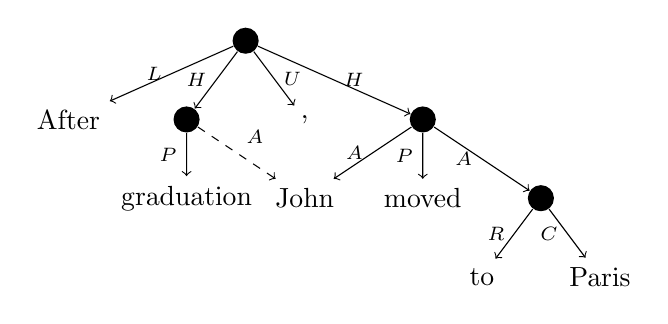
\begin{tikzpicture}[level distance=10mm, ->]
    \node (ROOT) [fill=black, circle] {}
      child {node (After) {After} edge from parent node[left] {\scriptsize $L$}}
      child {node (graduation) [fill=black, circle] {}
      {
        child {node {graduation} edge from parent node[left] {\scriptsize $P$}}
      } edge from parent node[left] {\scriptsize $H$} }
      child {node {,} edge from parent node[right] {\scriptsize $U$}}
      child {node (moved) [fill=black, circle] {}
      {
        child {node (John) {John} edge from parent node[left] {\scriptsize $A$}}
        child {node {moved} edge from parent node[left] {\scriptsize $P$}}
        child {node [fill=black, circle] {}
        {
          child {node {to} edge from parent node[left] {\scriptsize $R$}}
          child {node {Paris} edge from parent node[left] {\scriptsize $C$}}
        } edge from parent node[left] {\scriptsize $A$} }
      } edge from parent node[right] {\scriptsize $H$} }
      ;
    \draw[dashed,->] (graduation) to node [auto] {\scriptsize $A$} (John);
  \end{tikzpicture}
  }}
  \end{subfigure}
  \begin{subfigure}[t]{.9\columnwidth}
  \parbox{.1\columnwidth}{\caption{}\label{fig:home}}
  \hspace{.1\columnwidth}
  \parbox{.7\columnwidth}{
  \scalebox{.9}{
  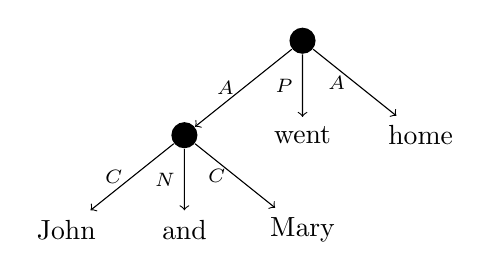
\begin{tikzpicture}[level distance=12mm, ->,
      every node/.append style={midway}]
    \node (ROOT) [fill=black, circle] {}
      child {node [fill=black, circle] {}
      {
        child {node {John} edge from parent node[left] {\scriptsize $C$}}
        child {node {and} edge from parent node[left] {\scriptsize $N$}}
        child {node {Mary} edge from parent node[left] {\scriptsize $C$}}
      } edge from parent node[left] {\scriptsize $A$} }
      child {node {went} edge from parent node[left] {\scriptsize $P$}}
      child {node {home} edge from parent node[left] {\scriptsize $A$}}
      ;
  \end{tikzpicture}
  }}
  \end{subfigure}
  \begin{subfigure}[t]{.9\columnwidth}
  \parbox{.1\columnwidth}{\caption{}\label{fig:gave}}
  \hspace{.25\columnwidth}
  \parbox{.55\columnwidth}{
  \scalebox{.9}{
  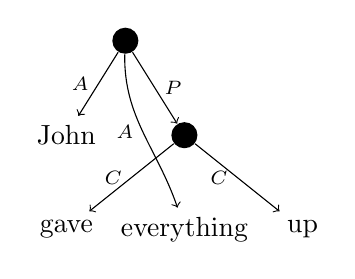
\begin{tikzpicture}[level distance=12mm, ->,
      every node/.append style={midway}]
    \node (ROOT) [fill=black, circle] {}
      child {node {John} edge from parent node[left] {\scriptsize $A$}}
      child {node [fill=black, circle] {}
      {
      	child {node {gave} edge from parent node[left] {\scriptsize $C$}}
      	child {node (everything) {everything} edge from parent[white]}
      	child {node {up} edge from parent node[left] {\scriptsize $C$}}
      } edge from parent node[right] {\scriptsize $P$} }
      ;
    \draw[bend right,->] (ROOT) to[out=-20, in=180] node [left] {\scriptsize $A$} (everything);
  \end{tikzpicture}
  }}
  \end{subfigure}
  \caption{\label{fig:examples}
    Semantic representation of the three structural properties
    required for BSS, according to the UCCA scheme. (\subref{fig:graduation}) includes a remote edge (dashed),
    resulting in ``John'' having two parents. % and a linkage relation (gray node and its outgoing edges).
    (\subref{fig:home}) includes a coordination construction (``John and Mary'').
    (\subref{fig:gave}) includes a discontinuous unit (``gave ... up'').
    Legend: $P$ -- a Scene's main relation, $A$ -- participant,
    $L$ -- inter-scene linker, $H$ -- linked Scene, $C$ -- center,
    $R$ -- relator, $N$ -- connector, $U$ -- punctuation, $F$ -- function unit.
    Pre-terminal nodes are omitted for brevity.
  }
\end{figure}

However, to our knowledge, no existing parser for a grounded semantic annotation scheme
supports the combination of these criteria.
The only such scheme supporting them is UCCA \cite{abend2013universal},
which has no parser.
Several other models either support some of these properties \cite{oepen2015semeval},
or avoid grounding semantic units altogether
(notably, AMR \cite{banarescu2013abstract}; see \secref{sec:related_work}).

In this work we are first in proposing techniques for BSS parsing.
We adopt a transition-based approach, which has recently produced some of the best
results in syntactic dependency parsing
\cite{dyer2015transition,ballesteros2015improved}, and has also demonstrated
strong performance in a variety of other semantic and syntactic settings
\cite[among others]{maier2015discontinuous,wang2015transition}.
Transition-based methods are a natural starting point for UCCA parsing,
as the set of distinctions it represents, centered around predicate-argument
structures and their inter-relations, is similar to distinctions
conveyed by dependency schemes.

We pursue two complementary parsing strategies.
First, we assess the ability of existing technology to tackle the task,
by developing conversion protocols between UCCA structures and two related formalisms:
dependency trees and discontinuous constituency trees.
As these formalisms are more restrictive than BSS, the conversion
is necessarily lossy. Nonetheless, we find that it is effective
in practice (\secref{sec:conversion_approach}).
Second, we present a novel transition-based broad-coverage parser,
Broad-coverage Semantic Parser (\textsc{bsp}; \secref{sec:direct_approach})
supporting multiple parents, non-terminal nodes and discontinuous units,
based on extending existing transition-based parsers
with new transitions and features.

We experiment with the English UCCA-annotated corpora \cite{abend2013universal}
as a test case, in both in-domain and out-of-domain scenarios, reaching
nearly 70\% labeled F-score for the highest scoring parser.
The results suggest concrete paths for further improvement.
All converters and parsers will be made publicly available upon publication.


%%%%%%%%%%%%%%%%%%%%%%%%%%%%%%%%%%%%%%%%%%%%%%%%%%%%%%%%%%%%%%%
\vspace{-.1cm}

\section{Related Work}\label{sec:related_work}
While earlier work on grounded semantic parsing has mostly concentrated on shallow semantic analysis,
focusing on semantic role labeling of verbal argument structures,
the focus has recently shifted to parsing of more elaborate representations that account
for a wider range of phenomena.


\paragraph{Broad-Coverage Semantic Parsing.}
Most closely related to this work is Broad-Coverage Semantic Dependency Parsing (SDP),
addressed in two SemEval tasks \cite{oepen2014semeval,oepen2015semeval},
experimenting with the Prague tectogrammatical layer \cite{sgallhp:1986,bohmova2003prague},
and with dependencies derived from the
Enju parser,\footnote{See \url{http://kmcs.nii.ac.jp/enju}} and Lingo ERG \cite{Flic:02}.
Like BSS parsing, SDP addresses a wide range of semantic phenomena,
and supports discontinuous units and multiple parents. However, SDP uses
bi-lexical dependencies, disallowing non-terminal nodes, and thus faces difficulties in supporting
structures that have no clear head, such as coordination \cite{Ivanova2012who}.


\paragraph{Abstract Meaning Representation.}
Another line of work addresses parsing into
non-grounded\footnote{By \textit{grounded} we mean the text tokens are directly
annotated as part of the representation,
as opposed to abstract formalisms approximating logical form, for example.}
semantic representation, notably Abstract Meaning Representation (AMR)
\cite{flanigan2014discriminative,vanderwende2015amr,pust2015parsing,artzi2015broad}. 
While sharing much of this work's motivation,
not grounding the representation in the text
complicates the parsing task, as it requires
that the alignment between words and logical symbols be automatically
(and imprecisely) detected.\footnote{Considerable technical effort has been invested in
the AMR alignment task under various approaches
\cite{flanigan2014discriminative,pourdamghani2014aligning,pust2015parsing}.}
Furthermore, grounding allows breaking down sentences into semantically meaningful sub-spans,
which is useful for many applications (see discussion in \newcite{fernandez2015parsing}).
\newcite{wang2015transition} applied a transition-based approach to AMR parsing.
Their method involved first syntactically parsing the input, and then converting
the result into AMR.


\paragraph{Grammar-Based Methods.}
Semantic parsing methods can be largely partitioned into grammar-based and grammarless methods.
Within the grammar-based literature, most work relied on Combinatory Categorial Grammar (CCG)
\cite{Steedman:00}, which allows computing semantic structure compositionally from the
syntactic derivations. Notable examples include the Boxer parser \cite{bos2005towards}
and the AMR parser by \newcite{artzi2015broad}.
Other examples include parsing with Hyperedge Replacement Grammars
\cite{jones2012semantics,chiang2013parsing,peng2015synchronous} and
graph grammars \cite{koller2015semantic}.
A different line of work takes a discriminative, grammarless approach,
pursuing either graph-based methods that predict the highest ranking graph
(tree or DAG) that satisfies a given set of constraints
(e.g., \newcite{flanigan2014discriminative} for AMR parsing)
or a transition-based method that builds the parse incrementally following a series of local
decisions \cite[and much subsequent work]{Nivre03anefficient}.
\daniel{other grammar-based formalisms like HPSG and TAG ungrounded compositional semantics
by positing elaborate theories of syntax-semantics interface.
we suggest a direct approach which is discriminative and grammar-less and makes less
theoretical commitments about the syntax-semantics interface}

Other approaches for semantic representation, such as MRS \cite{copestake2005minimal}
and DRT \cite{kamp2011discourse},
involve considerably different representation and parsing approaches,
and so fall beyond the scope of our discussion.


%%%%%%%%%%%%%%%%%%%%%%%%%%%%%%%%%%%%%%%%%%%%%%%%%%%%%%%%%%%%%%%
\vspace{-.1cm}
\section{The UCCA Scheme}\label{sec:ucca}
Universal Conceptual Cognitive Annotation (UCCA)
is a cross-linguistically applicable semantic representation scheme,
that builds on the established ``Basic Linguistic Theory'' framework for typological description
\cite{Dixon:10b,Dixon:10a,Dixon:12}, and on the Cognitive Linguistics literature.
UCCA is a multi-layered representation, where each layer corresponds to a ``module'' of
semantic distinctions (e.g., predicate-argument structures, adverbials, coreference etc.).

Formally, a UCCA structure over a sentence is a DAG, whose leaves correspond to the sentence's words.
The nodes of the graph, or its ``units'', are either terminals or several
sub-units (not necessarily contiguous) jointly viewed as a
single entity according to some semantic or cognitive consideration.
Edges bear a category, indicating the role of the sub-unit in the relation that the parent represents.
UCCA structures support all three criteria of BSS: multiple parents, non-terminal nodes, and
discontinuous units.

UCCA's foundational layer, which we use here, covers the predicate-argument
structures evoked by predicates of all grammatical categories
(verbal, nominal, adjectival and others), the inter-relations between them,
as well as other major linguistic phenomena such as coordination and multi-word expressions.
This set of categories has demonstrated applicability to multiple languages, including
English, French, German and Czech, support for rapid annotation, and semantic stability in translation:
UCCA annotations of translated text usually contain the same set of relationships
\cite{sulem2015conceptual}. This finding supports the claim that UCCA represents an abstract
level of semantics, shared by different languages.

The layer's basic notion is the {\it Scene}, which describes a movement, action or state.
Each Scene contains one Main Relation, as well as one or more Participants.
For example, the sentence ``After graduation, John moved to Paris'' contains two Scenes,
whose main relations are ``graduation'' and ``moved''. ``John'' is a Participant in both Scenes,
while ``Paris'' only in the latter.
UCCA marks one of the incoming edges for each non-root
as ``primary'' and the others as ``remote'' edges.
The two Scenes in this sentence are both arguments of the \textit{Linker} ``After'',
which in this case expresses a temporal relation between them.
\figref{fig:examples} presents the UCCA annotation of this and other examples.

Further categories account for relations between Scenes and the internal structures of
complex arguments (e.g., coordination) and relations
(e.g., complex adverbials, such a ``very clearly''). UCCA graphs may contain implicit
units that have no correspondent in the text, but the parsing of these
units is deferred to future work, as it is likely to require different methods
than those explored here \cite{roth2015inducing}.



%%%%%%%%%%%%%%%%%%%%%%%%%%%%%%%%%%%%%%%%%%%%%%%%%%%%%%%%%%%%%%%
\section{Conversion-Based Parsing}\label{sec:conversion_approach}

We begin by assessing the ability of existing technology to address the task,
by taking a conversion-based approach.
Training proceeds by converting BSS into a different representation,
and training an existing parser on the converted structures.
We evaluate the trained parsers by applying them to the test set,
and converting the results back to BSS, where they are compared
with the gold standard.
Due to the success of dependency tree parsers, a similar approach has yielded
very strong parsers for other graph structures,
more general than dependency trees but not as general as BSS
\cite{agic2015semantic,fernandez2015parsing}, despite lossy reconstruction algorithms.
The error resulting from this back and forth conversion is discussed in
\secref{sec:results}.

\paragraph{Notation.}
Let $L$ be the set of possible edge labels.
A BSS is a directed acyclic graph $G=(V,E, \ell)$
over a sequence of tokens $w_1, \ldots, w_n$,
where $\ell:E\to L$ is a function of \textit{edge labels}.
For each token $w_i$ ($i=1, \ldots, n$), there exists a leaf (or a terminal) $t_i \in V$.

\paragraph{Conversion to Constituency Trees.}
We convert BSS to constituency trees by removing a subset of the
edges.\footnote{For trees, labeling nodes is equivalent to labeling edges. Thus,
  we do not distinguish between the two options. 
  Note also that as the original structures may contain discontinuities, so may the resulting trees.}
Specifically, when converting UCCA structures, we simply remove all remote edges,
leaving only primary edges, which form a tree structure (see \figref{fig:graduation}).
The inverse conversion from trees to BSS is simply the identity function, as every constituency tree is a BSS.

\paragraph{Conversion to Dependency Trees.}\label{subsec:con2dep}
In the conversion to dependency trees, we first convert BSS
to constituency trees using the above procedure, and then convert the result to dependency trees. 
Assume $T_c=(V_c,E_c,\ell_c)$ is a constituency tree with labels $\ell_c:E_c~\rightarrow~L$,
where $L$ is the set of possible labels.
The conversion from $T_c$ to a dependency tree involves the removal of
all non-terminals from $T_c$ and the addition of edges between terminals.
The nodes of the converted dependency tree are simply the terminals of $T_c$.

We define a linear order over possible edge labels $L$.
For each node $u \in V$, denote with $h(u)$ its child with the highest edge label.
Denote with $h^*(u)$ the terminal reached by recursively applying $h(\cdot)$ over $u$.
For each terminal $t$, we define $n(t)$ as the highest
non-terminal such that $t=h^*(n(t))$, i.e.,
$n(t)$ is the only node such that $t=h^*(n(t))$ and $t \neq h^*(\mathrm{Parent}_c(n(t)))$.
The head of $t$ according to the dependency graph is
the terminal $h^*(\mathrm{Parent}_c(n(t)))$.
The complete conversion procedure from constituency to dependency is given in Algorithm~\ref{alg:con2dep}.

We note that this conversion procedure is simpler than the
head percolation procedure used for converting syntactic constituency
trees to dependency trees.
This is because $h(u)$ of a node $u$ (similar to $u$'s head-containing child),
depends only on the label of the edge $(h(u),u)$, and not on the sub-tree spanned by $u$,
because edge labels in UCCA directly express the role of the child in the parent unit, and
are thus sufficient for determining which of $u$'s children contains the head node.

\begin{algorithm}[t]
  \small
  \KwData{constituency tree ${T_c}=(V_c,E_c,\ell_c)$}
 \KwResult{dependency tree $T_d=(V_d,E_d,\ell_d)$}
 \ForEach{$u \in V_c$} {
  $h(u) \leftarrow \argmin_v \mathrm{Priority}(\ell_c(u,v))$\;
 }
 $V_d \leftarrow \mathrm{Terminals}({T_c})$,
 $E_d \leftarrow \emptyset$\;
 \ForEach{$t \in V_d$} {
  $u \leftarrow t$\;
  \While{$u=h(\mathrm{Parent}_c(u))$} {
  	$h^*(u) \leftarrow t$\;
  	$u \leftarrow \mathrm{Parent}_c(u)$\;
  }
  $n(t) \leftarrow h(u)$\;
 }
 \ForEach{$t \in V_d$} {
  $u \leftarrow \mathrm{Parent}_c(n(t))$\;
  $t^\prime \leftarrow h^*(u)$\;
  $E_d \leftarrow E_d \cup \{(t^\prime, t)\}$\;
  $\ell_d (t^\prime, t) \leftarrow \ell_c(u, n(t))\}$\;
 }
 \caption{\small Constituency to dependency conversion procedure.}
 \label{alg:con2dep}
\end{algorithm}

The inverse conversion introduces non-terminal nodes back into the tree.
As the distinction between low- and high-attaching nodes is lost in the constituency to
dependency conversion, we heuristically assume that attachments are always
high-attaching.
Assume $T_d=(V_d,E_d,\ell_d)$ is a dependency tree.
We begin by creating a root node $r$.
Then, iterating over $V_d$ in topological order,
we add its members as terminals to the constituency tree
and create a pre-terminal parent for each,
with an edge labeled as \textit{Terminal} between them.
The parents of the pre-terminals are determined by the terminal's parent in the dependency
tree: if a dependency node $t$ is a child of the root in $T_d$, then $t$'s pre-terminal will also be a child of the root node. Otherwise, $t$'s pre-terminal is the child of the pre-terminal associated with $t$'s head in $T_d$. We add an intermediate node in between if $t$ has any dependents in $T_d$,
to allow adding their pre-terminals as children.
Edge labels for the intermediate edges are determined by a rule-based function, denoted by $\mathrm{Label}(u)$.\footnote{See Supplementary Material for the definition of $\mathrm{Label}$.}
In practice, it mostly selects the UCCA label \textit{Center}.
This conversion procedure is given in Algorithm~\ref{alg:dep2con}.

\begin{algorithm}[t]
  \small
 \KwData{dependency tree $T_d=(V_d,E_d,\ell_d)$}
 \KwResult{constituency tree $T_c=(V_c,E_c,\ell_c)$}
 $r \leftarrow \mathrm{Node()}$\;
 $V_c \leftarrow \{r\}$,
 $E_c \leftarrow \emptyset$\;
 \ForEach{$t \in \mathrm{TopologicalSort}(V_d)$} {
  $u \leftarrow \mathrm{Node()}$\;
  $V_c \leftarrow V_c \cup \{u, t\}$\;
  $E_c \leftarrow E_c \cup \{(u, t)\}$\;
  $\ell_c(u,t)\leftarrow\mathit{Terminal}$\;
  $t^\prime \leftarrow \mathrm{Parent}_d(t)$\;
  \eIf{$t^\prime = \textsc{Root}$} {
   $E_c \leftarrow E_c \cup \{(r, u)\}$\;
   $\ell_c(r, u) \leftarrow \mathrm{Label}(r)$\;
  } {
   \eIf{$\exists v \in V_d : (t,v) \in E_d$} {
    $u^\prime \leftarrow \mathrm{Node()}$\;
    $E_c \leftarrow E_c \cup \{(u^\prime, u)\}$\;
    $\ell_c(u^\prime, u) \leftarrow \mathrm{Label}(u^\prime)$\;
   } {
    $u' \leftarrow u$\;
   }
   $p \leftarrow \mathrm{Parent}_c(t^\prime)$\;
   $E_c \leftarrow E_c \cup \{(p, u^\prime)\}$\;
   $\ell_c(p, u^\prime) \leftarrow \ell_d(t^\prime, t)$\;
  }
 }
 \caption{\small Dependency to constituency conversion procedure.}
 \label{alg:dep2con}
\end{algorithm}


%%%%%%%%%%%%%%%%%%%%%%%%%%%%%%%%%%%%%%%%%%%%%%%%%%%%%%%%%%%%%%%
\section{Broad-Coverage Semantic Parsing}\label{sec:direct_approach}

We now turn to presenting \textsc{bsp},
a transition-based parser that supports the three criteria of broad-coverage
semantic structures.

Transition-based parsing \cite{Nivre03anefficient} creates the parse
as it scans the text from left to right.
The parse is created incrementally by applying a \textit{transition} at each step to the parser state,
defined using three data structures: a buffer $B$ of tokens and nodes to be processed,
a stack $S$ of nodes currently being processed,
and a graph $G=(V,E,\ell)$ of constructed nodes and labeled edges.
Some of the states are marked as \textit{terminal}, meaning that $G$ is the final output.
A classifier is used at each step to select the next transition based on features
that encode the parser's current state.
During training, an oracle creates training instances for the classifier,
based on the gold-standard annotation.

Despite being based on local decisions, transition-based methods have yielded excellent
results in a variety of parsing tasks.
Within syntactic dependency parsing, transition-based methods
have been successfully applied to corpora in many languages and domains, yielding some
of the best reported results \cite{dyer2015transition,ballesteros2015improved}. 
The approach has also yielded results comparable with the state-of-the-art in
constituency parsing \cite{sagae2005classifier,zhang2009transition,zhu2013fast},
discontinuous constituency parsing \cite{maier2015discontinuous},
as well as dependency DAG structures
\cite{sagae2008shift,tokgoz2015transition}, CCG structures \cite{ambati2015incremental}
and AMR parsing \cite{wang2015transition}.

\textsc{bsp} mostly builds on recent advances in discontinuous constituency
and dependency DAG parsing techniques, and further introduces novel UCCA-oriented features for parsing BSS.

\paragraph{Transition Set.}
Given a sequence of tokens $w_1, \ldots, w_n$, we predict a BSS $G$ whose leaves
correspond to the tokens. % $w_1, \ldots, w_n$.
Parsing starts with a single node on the stack (the root node), and the input tokens
$w_1, \ldots, w_n$ in the buffer. The set of transitions is given in \figref{fig:transitions}.
In addition to the standard \textsc{Shift} and \textsc{Reduce} operations, 
we follow previous work in transition-based constituency parsing \cite{sagae2005classifier}, and include the \textsc{Node} transition for creating new non-terminal nodes.
Concretely, \textsc{Node$_X$} creates a new node on the buffer as a parent of the first element on the stack, with an $X$-labeled edge.


\begin{figure*}
\begin{adjustbox}{width=\textwidth,margin=3pt,frame}
\begin{tabular}{llll|l|llllc|c}
\multicolumn{5}{c|}{\textbf{\small Initial State}} & \multicolumn{6}{c}{\textbf{\small Final State}} \\
\textbf{\footnotesize Stack} & \textbf{\footnotesize Buffer} & \textbf{\footnotesize Nodes} & \multicolumn{1}{l}{\textbf{\footnotesize Edges}} & \multicolumn{1}{c|}{\textbf{\footnotesize Terminal?}} & \textbf{\footnotesize Stack} & \textbf{\footnotesize Buffer} & \textbf{\footnotesize Nodes} & \textbf{\footnotesize Edges} & \multicolumn{1}{c}{\textbf{\footnotesize Terminal?}} \\
$[\mathrm{root}]$ & $w_{1:n}$ & \multirow{2}{40pt}{$\{\mathrm{root}\} \cup w_{1:n}$} & \multicolumn{1}{l}{$\emptyset$} & \multicolumn{1}{c|}{$-$} & $\emptyset$ & $\emptyset$ & $V$ & $E$ & \multicolumn{1}{c}{$+$} \\ 
\multicolumn{5}{c|}{} \\
\multicolumn{5}{c|}{} \\
\hline
\multicolumn{4}{c|}{\textbf{\small Before Transition}} & \textbf{\small Transition} & \multicolumn{5}{c|}{\textbf{\small After Transition}} & \textbf{\small Condition} \\
\textbf{\footnotesize Stack} & \textbf{\footnotesize Buffer} & \textbf{\footnotesize Nodes} & \textbf{\footnotesize Edges} & & \textbf{\footnotesize Stack} & \textbf{\footnotesize Buffer} & \textbf{\footnotesize Nodes} & \textbf{\footnotesize Edges} & \textbf{\footnotesize Terminal?} & \\
$S$ & $x \;|\; B$ & $V$ & $E$ & \textsc{Shift} & $S \;|\; x$ & $B$ & $V$ & $E$ & $-$ & \\
$S \;|\; x$ & $B$ & $V$ & $E$ & \textsc{Reduce} & $S$ & $B$ & $V$ & $E$ & $-$ & \\
$S \;|\; x$ & $B$ & $V$ & $E$ & \textsc{Node$_X$} & $S \;|\; x$ & $y \;|\; B$ & $V \cup \{ y \}$ & $E \cup \{ (y,x)_X \}$ & $-$ &
$x \neq \mathrm{root}$ \\
$S \;|\; y,x$ & $B$ & $V$ & $E$ & \textsc{Left-Edge$_X$} & $S \;|\; y,x$ & $B$ & $V$ & $E \cup \{ (x,y)_X \}$ & $-$ &
\multirow{4}{50pt}{\vspace{-5mm}\[\left\{\begin{array}{l}
x \not\in w_{1:n},\\
y \neq \mathrm{root},\\
y \not\leadsto_G x
\end{array}\right.\]} \\
$S \;|\; x,y$ & $B$ & $V$ & $E$ & \textsc{Right-Edge$_X$} & $S \;|\; x,y$ & $B$ & $V$ & $E \cup \{ (x,y)_X \}$ & $-$ & \\
$S \;|\; y,x$ & $B$ & $V$ & $E$ & \textsc{Left-Remote$_X$} & $S \;|\; y,x$ & $B$ & $V$ & $E \cup \{ (x,y)_X^* \}$ & $-$ & \\
$S \;|\; x,y$ & $B$ & $V$ & $E$ & \textsc{Right-Remote$_X$} & $S \;|\; x,y$ & $B$ & $V$ & $E \cup \{ (x,y)_X^* \}$ & $-$ & \\
$S \;|\; x,y$ & $B$ & $V$ & $E$ & \textsc{Swap} & $S \;|\; y$ & $x \;|\; B$ & $V$ & $E$ & $-$ &
$\mathrm{i}(x) < \mathrm{i}(y)$ \\
$[\mathrm{root}]$ & $\emptyset$ & $V$ & $E$ & \textsc{Finish} & $\emptyset$ & $\emptyset$ & $V$ & $E$ & $+$ & \\
\end{tabular}
\end{adjustbox}
\caption{\label{fig:transitions}
  The transition set of \textsc{bsp}. %Following standard practice,
  We write the stack with its top to the right and the buffer with its head to the left.
  $(\cdot,\cdot)_X$ denotes a primary $X$-labeled edge, and $(\cdot,\cdot)_X^*$ a remote $X$-labeled edge.
  $\mathrm{i}(x)$ is a running index for the created nodes.
  \textsc{Edge} transitions have an additional condition: the prospective child may not
  already have a primary parent.
}
\end{figure*}

\textsc{Left-Edge$_X$} and \textsc{Right-Edge$_X$} create a new primary $X$-labeled edge between the first two elements on the stack, where the parent is the left or the right node, respectively. As a UCCA node may only
have one incoming primary edge, \textsc{Edge} transitions are disallowed where the child node already
has an incoming primary edge.
\textsc{Left-Remote$_X$} and \textsc{Right-Remote$_X$} do not have this restriction, and the created edge is
marked as \textit{remote}. We distinguish between these two pairs of transitions, for the parser
to be able to determine whether an edge is a primary or a remote one.
In order to support the prediction of multiple parents, node and edge transitions do not automatically
apply \textsc{Reduce}. This is in line with other work on
transition-based DAG dependency parsing \cite{sagae2008shift,tokgoz2015transition}.
Once all edges for a particular node have been created, it is removed from the stack
by applying \textsc{Reduce}.

\textsc{Swap} allows handling discontinuous nodes, by popping the second
node on the stack and adding it to the top of the buffer, as with the similarly
named transition in previous work \cite{nivre2009non,maier2015discontinuous}.
Finally, \textsc{Finish} pops the root node and marks the state as terminal.

\paragraph{Features.}
\label{subsec:features}

\figref{fig:features} presents the feature templates used by the parser.
For some of the features, we used the notion of \textit{head word},
defined by the $h^*(\cdot)$ function (\secref{subsec:con2dep}).
While head words are not explicitly represented in the UCCA scheme, these
features proved useful as means of encoding word-to-word relations.

In addition to the binary features defined by the feature templates,
we employ a real-valued feature, \textbf{ratio}, corresponding to the ratio between the number of terminals to number of nodes
in the graph $G$. This novel feature serves as a regularizer for the creation of new nodes, and should be beneficial for other transition-based constituency parsers too.
Features are generally adapted from the related parsers of \cite{zhang2009transition,zhu2013fast,tokgoz2015transition,maier2015discontinuous}, with a small additional set of features encoding relevant information
for the novel \textsc{Left-Remote$_X$} and \textsc{Right-Remote$_X$} transitions.

% FEATURES
\begin{figure}
  \begin{adjustbox}{margin=3pt,frame}

\begin{tabular}{>{\small}l}
{Features from \cite{zhang2009transition}:} \\
\textbf{unigrams} \\
$s_0te, s_0we, s_1te, s_1we, s_2te, s_2we, s_3te, s_3we,$ \\
$b_0wt, b_1wt, b_2wt, b_3wt,$ \\
$s_0lwe, s_0rwe, s_0uwe, s_1lwe, s_1rwe, s_1uwe$ \\
\textbf{bigrams} \\
$s_0ws_1w, s_0ws_1e, s_0es_1w, s_0es_1e, s_0wb_0w, s_0wb_0t,$ \\
$s_0eb_0w, s_0eb_0t, s_1wb_0w, s_1wb_0t, s_1eb_0w, s_1eb_0t,$ \\
$b_0wb_1w, b_0wb_1t, b_0tb_1w, b_0tb_1t$ \\
\textbf{trigrams} \\
$s_0es_1es_2w, s_0es_1es_2e, s_0es_1eb_0w, s_0es_1eb_0t,$ \\
$s_0es_1wb_0w, s_0es_1wb_0t, s_0ws_1es_2e, s_0ws_1eb_0t$ \\
\textbf{separator} \\
$s_0wp, s_0wep, s_0wq, s_0wcq, s_0es_1ep, s_0es_1eq,$ \\
$s_1wp, s_1wep, s_1wq, s_1weq$ \\
\\
\textbf{extended} \cite{zhu2013fast} \\
$s_0llwe, s_0lrwe, s_0luwe, s_0rlwe, s_0rrwe,$ \\
$s_0ruwe, s_0ulwe, s_0urwe, s_0uuwe, s_1llwe,$ \\
$s_1lrwe, s_1luwe, s_1rlwe, s_1rrwe, s_1ruwe$ \\
\\
\textbf{disco} \cite{maier2015discontinuous} \\
$s_0xwe, s_1xwe, s_2xwe, s_3xwe,$ \\
$s_0xte, s_1xte, s_2xte, s_3xte,$ \\
$s_0xy, s_1xy, s_2xy, s_3xy$ \\
$s_0xs_1e, s_0xs_1w, s_0xs_1x, s_0ws_1x, s_0es_1x,$ \\
$s_0xs_2e, s_0xs_2w, s_0xs_2x, s_0ws_2x, s_0es_2x,$ \\
$s_0ys_1y, s_0ys_2y, s_0xb_0t, s_0xb_0w$ \\
\\
{\footnotesize Features from \cite{tokgoz2015transition}:} \\
\textbf{counts} \\
$s_0P, s_0C, s_0wP, s_0wC, b_0P, b_0C, b_0wP, b_0wC$ \\
\textbf{edges} \\
$s_0s_1, s_1s_0, s_0b_0, b_0s_0, s_0b_0e, b_0s_0e$ \\
\textbf{history} \\
$a_0we, a_1we$ \\
\\
\textbf{remote} (Novel, UCCA-specific features) \\
$s_0R, s_0wR, b_0R, b_0wR$
\end{tabular}
\end{adjustbox}

\caption{\label{fig:features}
  Feature templates for \textsc{bsp}. Notation:
  $s_i$, $b_i$ are the $i$th stack and buffer items, respectively.
  $w$ and $t$ are the word form and part-of-speech tag of the terminal returned by the $h^*(\cdot)$ function (\secref{subsec:con2dep}).
  $e$ is the edge label to the node returned by the $h(\cdot)$ function.
  $l$, $r$ ($ll$, $rr$) are the leftmost and rightmost (grand)children, respectively.
  $u$ ($uu$) is the unary (grand)child, when only one exists.
  $p$ is a unique separator punctuation and $q$ is the separator count between $s_0$ and $s_1$.
  $x$ is the gap type (``none'', ``pass'' or ``gap'') at the sub-graph under the current node, and $y$ is the sum of gap lengths \protect\cite{Maier:Lichte:11}.
  $P$ and $C$ are the number of parents and children, respectively, and $R$ is the number of remote children.
  $a_i$ is the transition taken $i$ steps back.
  All feature templates correspond to binary features.
}
\end{figure}

\paragraph{Training.}
Following \newcite{maier2015discontinuous}, we use a linear classifier, using
the averaged structured perceptron algorithm for training it
\cite{Coll:04} with the \textsc{MinUpdate} \cite{goldberg2011learning} procedure:
a minimum number of updates to a feature has to occur in training for it
to be included in the model. Inference is performed greedily (i.e., without beam search).

For training the local classifier, we use a dynamic oracle \cite{goldberg2012dynamic},
i.e., an oracle that outputs a set of optimal transitions: when
applied to the current parser state, the gold
standard graph is reachable from the resulting state.
For example, the oracle would predict a \textsc{Node} transition if the stack 
has on its top a parent in the gold graph that has not been created,
but would predict a \textsc{Right-Edge} transition if the second stack
element is a parent of the
first element according to the gold graph and the edge between them has not been created.
The transition predicted by the classifier is deemed correct
and is applied to the parser state to reach the subsequent state,
if the transition is included in the set of optimal transitions.
Otherwise, a random optimal transition is applied
and the classifier's weights are updated according to the perceptron
update rule.



%%%%%%%%%%%%%%%%%%%%%%%%%%%%%%%%%%%%%%%%%%%%%%%%%%%%%%%%%%%%%%%
%\section{Experiments}\label{sec:experiments}

%%%%%%%%%%%%%%%%%%%%%%%%%%%%%%%%%%%%%%%%%%%%%%%%%%%%%%%%%%%%%%%
\section{Experimental Setup}\label{sec:exp_setup}

\paragraph{Data.}\label{sec:data}
We conduct our main experiments on the UCCA Wikipedia corpus (henceforth, \textit{Wiki}),
and use the English part of the UCCA \textit{Twenty Thousand Leagues Under the Sea} English-French parallel corpus (henceforth, \textit{20K Leagues}) as
out-of-domain data.\footnote{Both are available at \url{http://www.cs.huji.ac.il/~oabend/ucca.html}}
\tabref{table:data} presents some statistics for the two corpora, demonstrating that while
the \textit{Wiki} corpus is over ten times larger, the overall statistics are
similar.
We use passages of indices up to 655
of the \textit{Wiki} corpus as our training set, passages 656--700 as development set,
and passages 701--695 as in-domain test set.
While UCCA edges can cross sentence boundaries, we adhere to the common
practice in semantic parsing and train our parsers on individual sentences,
discarding inter-relations between them (0.18\% of the edges).
We also discard linkage nodes and edges, as they often express inter-sentence
relations and are thus mostly redundant when applied at the sentence level,
as well as implicit nodes (\secref{sec:ucca}).
In the out-of-domain experiments, we apply the same parser
(trained on the \textit{Wiki} corpus) to the \textit{20K Leagues} corpus
without re-tuning the parameters.


\begin{table}
  \scalebox{.8}{
\begin{tabular}{l|ccc|c}
& \multicolumn{3}{c|}{Wiki} & 20K \\
& \small Train & \small Dev & \small Test & Leagues \\
\hline
\# passages & 281 & 35 & 43 & 154 \\
\# sentences & 4021 & 537 & 608 & 522 \\
\hline
\# nodes & 277,587 & 40,700 & 45,047 & 29,965 \\
\% terminal & 42.41 & 42.8 & 42.66 & 41.23 \\
\% non-term. & 57.59 & 57.20 & 57.34 & 58.77 \\
\% implicit & 0.29 & 0.35 & 0.27 & 0.8 \\
\% linkage & 0.92 & 0.96 & 0.9 & 1.25 \\
\% discont. & 0.52 & 0.55 & 0.47 & 0.79 \\
\% \textgreater 1 parent & 2.29 & 1.89 & 2.21 & 1.98 \\
\hline
\# edges & 272,018 & 39,660 & 44,139 & 28,723 \\
\% primary & 95.37 & 95.70 & 95.90 & 94.48 \\
\% remote & 1.69 & 1.24 & 1.32 & 2.19 \\
\% linkage & 2.94 & 3.06 & 2.78 & 3.33 \\
\hline
\multicolumn{3}{l}{\footnotesize Average per non-linkage non-terminal node} \\
%\# parents & 0.98 & 0.97 & 0.98 & 0.95 \\
\# children & 1.67 & 1.67 & 1.67 & 1.61 
\end{tabular}
}
\caption{Statistics of the \textit{Wiki} and \textit{20K Leagues} UCCA corpora.
All counts exclude the root node.
}
\label{table:data}
\end{table}

\paragraph{Evaluation.}
Since there are no standard evaluation measures for BSS, we define
two simple measures for comparing such structures.
Assume $G_p=(V_p,E_p,\ell_p)$ and $G_g=(V_g,E_g,\ell_g)$
are the predicted and gold-standard DAGs over the same
sequence of terminals $W = \{w_1,\ldots,w_n\}$, respectively.
For an edge $e=(u,v)$ in either graph,
where $u$ is the parent and $v$ is the child, define its yield $y(e) \subseteq W$ as the
set of terminals in $W$ that are descendants of $v$.
We define the set of \textit{mutual edges} between $G_p$ and $G_g$:

\vspace{-.6cm}

{\small
\begin{multline*}
    M(G_p,G_g) = \\
    \left\{(e_1,e_2) \in E_p \times E_g \;|\;
    y(e_1) = y(e_2) \wedge \ell_p(e_1)=\ell_g(e_2)\right\}
\end{multline*}
}

\vspace{-.6cm}

Labeled precision and recall are defined by dividing $|M(G_p,G_g)|$ by $|E_p|$ and $|E_g|$, respectively.
We report two variants of this measure, one where we consider only non-remote edges,
and another where we consider remote edges. We note that the measure collapses to the standard
PARSEVAL constituency evaluation measure if $G_p$ are $G_g$ are trees.
Punctuation marks are excluded from the evaluation, but not from the datasets.

\paragraph{Conversions.}
We explore two conversion scenarios: one into (possibly discontinuous) constituency trees,
and one into CoNLL-style dependencies. In the first setting we experiment with \textsc{uparse},
the only transition-based constituency parser, to our knowledge, able to parse trees with
discontinuous constituents.
In the second setting we use the MaltParser with arc-standard and
arc-eager transition sets \cite{nivre2007maltparser},\footnote{Preliminary
experiments with non-projective variants of MaltParser yielded lower scores than
projective ones, and were thus discarded from the final evaluation.}
and the stack LSTM-based arc-standard parser \cite{dyer2015transition}.
For MaltParser, we try both SVM and perceptron classifiers, reporting
results obtained with SVM (about 1\% F-score higher).
Default settings are used in all cases.
We do not use existing dependency DAG parsers since we could not obtain their code.
We note that \textsc{uparse} uses beam search by default,
with a beam size of 4, where the other parsers use greedy search.

Upper bounds for the conversion-based methods are computed by applying
the conversion and inverse conversion on the gold standard
graphs and comparing them to the original gold standard.

\paragraph{\textsc{bsp}.}
We train \textsc{bsp} for 16 iterations, using $\textsc{MinUpdate}=5$
and $\textsc{Importance}=2$, doubling weight updates
for gold \textsc{Swap} transitions to address the sparseness
of discontinuous structures, as in \newcite{maier2015discontinuous}.
We train \textsc{bsp} both with and without remote edge transitions,
to allow better comparison with conversion-based methods that only
predict trees.

%%%%%%%%%%%%%%%%%%%%%%%%%%%%%%%%%%%%%%%%%%%%%%%%%%%%%%%%%%%%%%%
\section{Results}\label{sec:results}

\tabref{table:results} presents the results of our main experiments, as well as
upper bounds for the conversion-based methods.
\textsc{bsp} obtains comparable F-scores to MaltParser and \textsc{uparse}
in terms of primary edges, but unlike them, is able to predict some
of the remote edges too. 
Removing remote edge transitions from \textsc{bsp} does not
change results considerably on the primary edges,
improving them by 0.9\% F-score in the in-domain setting, but reduces
them by the same amount when applied out-of-domain. 
Out-of-domain results are largely comparable with the in-domain
results, demonstrating robustness by \textsc{bsp}
to domain variation.

The LSTM parser obtains the highest primary F-score,
with a considerable margin. Importantly, it obtains 9.1\%
F-score higher than the arc-standard MaltParser,
differing from it only in its classifier.
This suggests that applying a similar approach to
\textsc{bsp} is likely to improve results,
and further underscores the effectiveness of transition-based 
methods for BSS parsing. 

The conversion to constituency format only removes remote edges,
and thus obtains a perfect primary edge score.
The conversion to dependency format loses considerably more information, since
all non-terminal nodes are lost and have to be reconstructed by a
simple rule-based inverse conversion. Both conversions yield zero scores on remote edges,
since these are invariably removed when converting to trees.

\begin{table}[ht]
  \scalebox{.8}{
\begin{tabular}{l|ccc|ccc}
& \multicolumn{3}{c|}{Primary} & \multicolumn{3}{c}{Remote} \\
& \textbf{LP} & \textbf{LR} & \textbf{LF} & \textbf{LP} & \textbf{LR} & \textbf{LF} \\
\hline
\multicolumn{4}{l}{\rule{0pt}{2ex} \footnotesize Constituency Tree Conversion} \\
\textsc{uparse} & 64 & 67.3 & 65.4 & $-$ & 0 & 0 \\
Upper Bound & 100 & 100 & 100 & $-$ & 0 & 0 \\
\hline
\multicolumn{4}{l}{\rule{0pt}{4ex} \footnotesize Dependency Tree Conversion} \\
Malt$_{\textrm{arc-standard}}$ & 63.4 & 57.3 & 60.1 & $-$ & 0 & 0 \\
Malt$_{\textrm{arc-eager}}$ & 63.9 & 57.9 & 60.5 & $-$ & 0 & 0 \\
LSTM & {\bf 73.2} & {\bf 66.2} & {\bf 69.2} & $-$ & 0 & 0 \\
Upper Bound & 93.8 & 83.7 & 88.4 & $-$ & 0 & 0 \\
\hline
\multicolumn{4}{l}{\rule{0pt}{4ex} \footnotesize Direct Approach} \\
\textsc{bsp} & 62.4 & 56 & 59 & 15.3 & 11.8 & 13.3 \\
\textsc{bsp}$_{\mathrm{Tree}}$ & 63.8 & 56.5 & 59.9 & $-$ & 0 & 0 \\
\hhline{=======}
\multicolumn{4}{l}{\rule{0pt}{4ex} \footnotesize Out-of-domain} \\
\textsc{bsp} & 60.6 & 53.9 & 57.1 & 20.2 & 10.3 & 13.6 \\
\textsc{bsp}$_{\mathrm{Tree}}$ & 60.2 & 52.8 & 56.2 & $-$ & 0 & 0 \\
\end{tabular}
}
\caption{
  Main experimental results in percents (on the \textit{Wiki} test set, except for the bottom part). Columns correspond to labeled precision,
  recall and F-score for the different parsers, for both primary (left-hand side)
  and remote (right-hand side) edges. Top: results for \textsc{uparse}
  after conversion to constituency tree annotation. Upper middle: results for the
  MaltParser arc-eager and arc-standard, and
  the LSTM parser, after conversion to dependency tree annotation.
  Lower middle: results for our \textsc{bsp}, when trained on the complete UCCA DAGs (\textsc{bsp}),
  and when trained on UCCA trees, obtained by removing remote edges (\textsc{bsp}$_{\mathrm{Tree}}$).
  Bottom: results for \textsc{bsp} and \textsc{bsp}$_{\mathrm{Tree}}$ when tested on out-of-domain data (\textit{20K Leagues}).
}
\label{table:results}
\end{table}

\paragraph{Feature Ablation.}
To evaluate the relative impact of the different feature sets on \textsc{bsp},
we remove a set of features at a time,
and evaluate the resulting parser on the development set (\tabref{table:ablation}).
Almost all feature sets have a positive contribution to the primary edge F-score, 
or otherwise to the prediction of remote edges.
\textbf{unigrams} and \textbf{bigrams} features are especially
important, and the \textbf{ratio} feature greatly improves recall on
primary edges. \textbf{disco} features have a positive contribution,
likely to be amplified in languages with a higher percentage of discontinuous units, e.g. German.

\begin{table}[ht]
  \scalebox{.8}{
\begin{tabular}{l|ccc|ccc}
& \multicolumn{3}{c|}{Primary} & \multicolumn{3}{c}{Remote} \\
& \textbf{LP} & \textbf{LR} & \textbf{LF} & \textbf{LP} & \textbf{LR} & \textbf{LF} \\
\hline
\textsc{bsp} & 62.6	& 55.7 & 58.9 & 20 & 12.9 & 15.7 \\
\textsc{bsp}$-$\textbf{unigrams} & 62.5 & 52.6 & 57.1 & 18.9 & 10.1 & 13.2 \\
\textsc{bsp}$-$\textbf{bigrams} & 59.8 & 50.0 & 54.4 & 18.2 & 12.2 & 14.6 \\
\textsc{bsp}$-$\textbf{trigrams} & 63.7 & 55.0 & 59.0 & 20.7 & 12.0 & 15.2 \\
\textsc{bsp}$-$\textbf{separator} & 62.9 & 53.5 & 57.8 & 17.8 & 11.7 & 14.1 \\
\textsc{bsp}$-$\textbf{extended} & 62.9 & 52.8 & 57.4 & 17.4 & 11.5 & 13.9 \\
\textsc{bsp}$-$\textbf{disco} & 63.6 & 53.6 & 58.2 & 19.7 & 11.5 & 14.5 \\
\textsc{bsp}$-$\textbf{counts} & 63.3 & 52.8 & 57.6 & 14.6 & 10.6 & 12.3 \\
\textsc{bsp}$-$\textbf{edges} & 63.5 & 54.9 & 58.9 & 23.6 & 14.5 & 17.9 \\
\textsc{bsp}$-$\textbf{history} & 63.1 & 53.2 & 57.8 & 23.7 & 14.5 & 18.0 \\
\textsc{bsp}$-$\textbf{remote} & 63.5 & 53.2 & 57.9 & 17.2 & 10.6 & 13.1 \\
\textsc{bsp}$-$\textbf{ratio} & 63.7 & 48.3 & 55.0 & 25.4 & 13.6 & 17.7
\end{tabular}
}
\caption{
  Results on the development set for the feature ablation experiment, in percents.
  The first row corresponds to \textsc{bsp} as in the main experiment.
  In each of the other rows, one feature set is excluded.
  Columns are the same as in \tabref{table:results}.
  See \secref{subsec:features} and \figref{fig:features} for the feature set definitions.
}
\label{table:ablation}
\end{table}



%%%%%%%%%%%%%%%%%%%%%%%%%%%%%%%%%%%%%%%%%%%%%%%%%%%%%%%%%%%%%%%
\section{Conclusion}\label{sec:conclusion}

We have introduced the first parser that supports multiple parents, non-terminal
nodes and discontinuous units.
We further explored a conversion-based parsing approach to assess the ability of existing
technology to address the task.
The work makes a further contribution by first experimenting on UCCA parsing.
Results show that UCCA can be parsed with 69.2\% primary F-score,
and suggest means for improvement by taking an LSTM-based
approach to the local classifier of \textsc{bsp}.
The quality of the results is underscored by UCCA's inter-annotator
agreement (often taken as an upper bound) of 
80--85\% F-score on primary edges \cite{abend2013universal}.


While much recent work focused on semantic parsing of different types,
the relations between the different representations have not been clarified.
We intend to further explore conversion-based parsing approaches,
including different target representations and more sophisticated conversion procedures \cite{kong-15},
to shed light on the commonalities and differences between representations, suggesting ways to
design better semantic representations.
We believe that UCCA's merits in providing a cross-linguistically applicable, broad-coverage
annotation will support ongoing efforts to incorporate deeper semantic structures
into a variety of applications, such as machine translation \cite{jones2012semantics}
and summarization \cite{liu2015toward}.


\bibliography{references}
\bibliographystyle{emnlp2016}

\end{document}
